
\section{Validation Metrics} 
\label{sec:validation-metrics}

There are various methods and algorithms available to evaluate the similarity between two or more seismograms, both through direct quantitative comparisons or indirect statistical analysis \citep[e.g.,][]{Anderson_2004_Proc, Kristekova_2006_BSSA, Kristekova_2009_GJI, Olsen_2010_SRL, Burks_BSSA_2014, Rezaeian_2015_BSSA}. In earthquake ground motion simulation, they are primarily used for verification with respect to benchmark or analytical solutions, and for validation with respect to data (i.e., ground motion records). Here, we focus on the list of metrics proposed by \citet{Anderson_2004_Proc}, with an additional metric for duration, as suggested by others \citep{Olsen_2010_SRL, Maufroy_2015_BSSA} and as implemented in \citet{Taborda_2013_BSSA}.


\begin{table}[t]
\caption{Validation Metrics}
\centering
\small
\begin{tabular}{ll}
	\hline
	\multicolumn{1}{c}{Code}          & 
	\multicolumn{1}{c}{Metric}        \\
	\hline
	C1   & Arias Intensity Integral   \\
	C2   & Energy Integral            \\
	C3   & Arias Intensity		      \\
	C4   & Total Energy               \\
	C5   & Peak Acceleration          \\
	C6   & Peak Velocity              \\
	C7   & Peak Displacement          \\
	C8   & Response Spectrum          \\
	C9   & Fourier Amplitude Spectrum \\
	C10  & Cross Correlation          \\
	C11  & Strong Phase Duration      \\
	\hline
\end{tabular}
\label{tab:metrics}
\end{table}


These metrics are listed in Table \ref{tab:metrics}. Following \citet{Anderson_2004_Proc}, when applied to a pair of signals, each one of these metrics yields a GOF score ranging from 0 to 10, where a value of 10 corresponds to two signals having identical characteristics. This scoring scale varies according to the following exponential function:
% 
\begin{equation}
\label{eq:gof-function}
	S \left( p_1, p_2 \right) = 10 \exp{ \left[ - \left( \frac{p_1 - p_2}{ \min\left( p_1, p_2 \right) } \right)^2 \right] }
	\, ,
\end{equation}
% 
\noindent
where $S$ is the GOF score that results from comparing values $p_1$ and $p_2$ from signals 1 and 2, respectively, for each one of the different metrics in Table \ref{tab:metrics}. \citeauthor{Anderson_2004_Proc} also provided guidelines for the process to be applied to the original signals as well as to those resulting from a sequential set of band-pass filters covering the whole frequency range of interest. In his method, this frequency-domain decomposition should have pass bands defined following a logarithmic distribution in order to give more weight to the low-frequencies, and the GOF scores of all sub-bands and the broadband be averaged into a single GOF final score.

\begin{figure*}
    \centering
    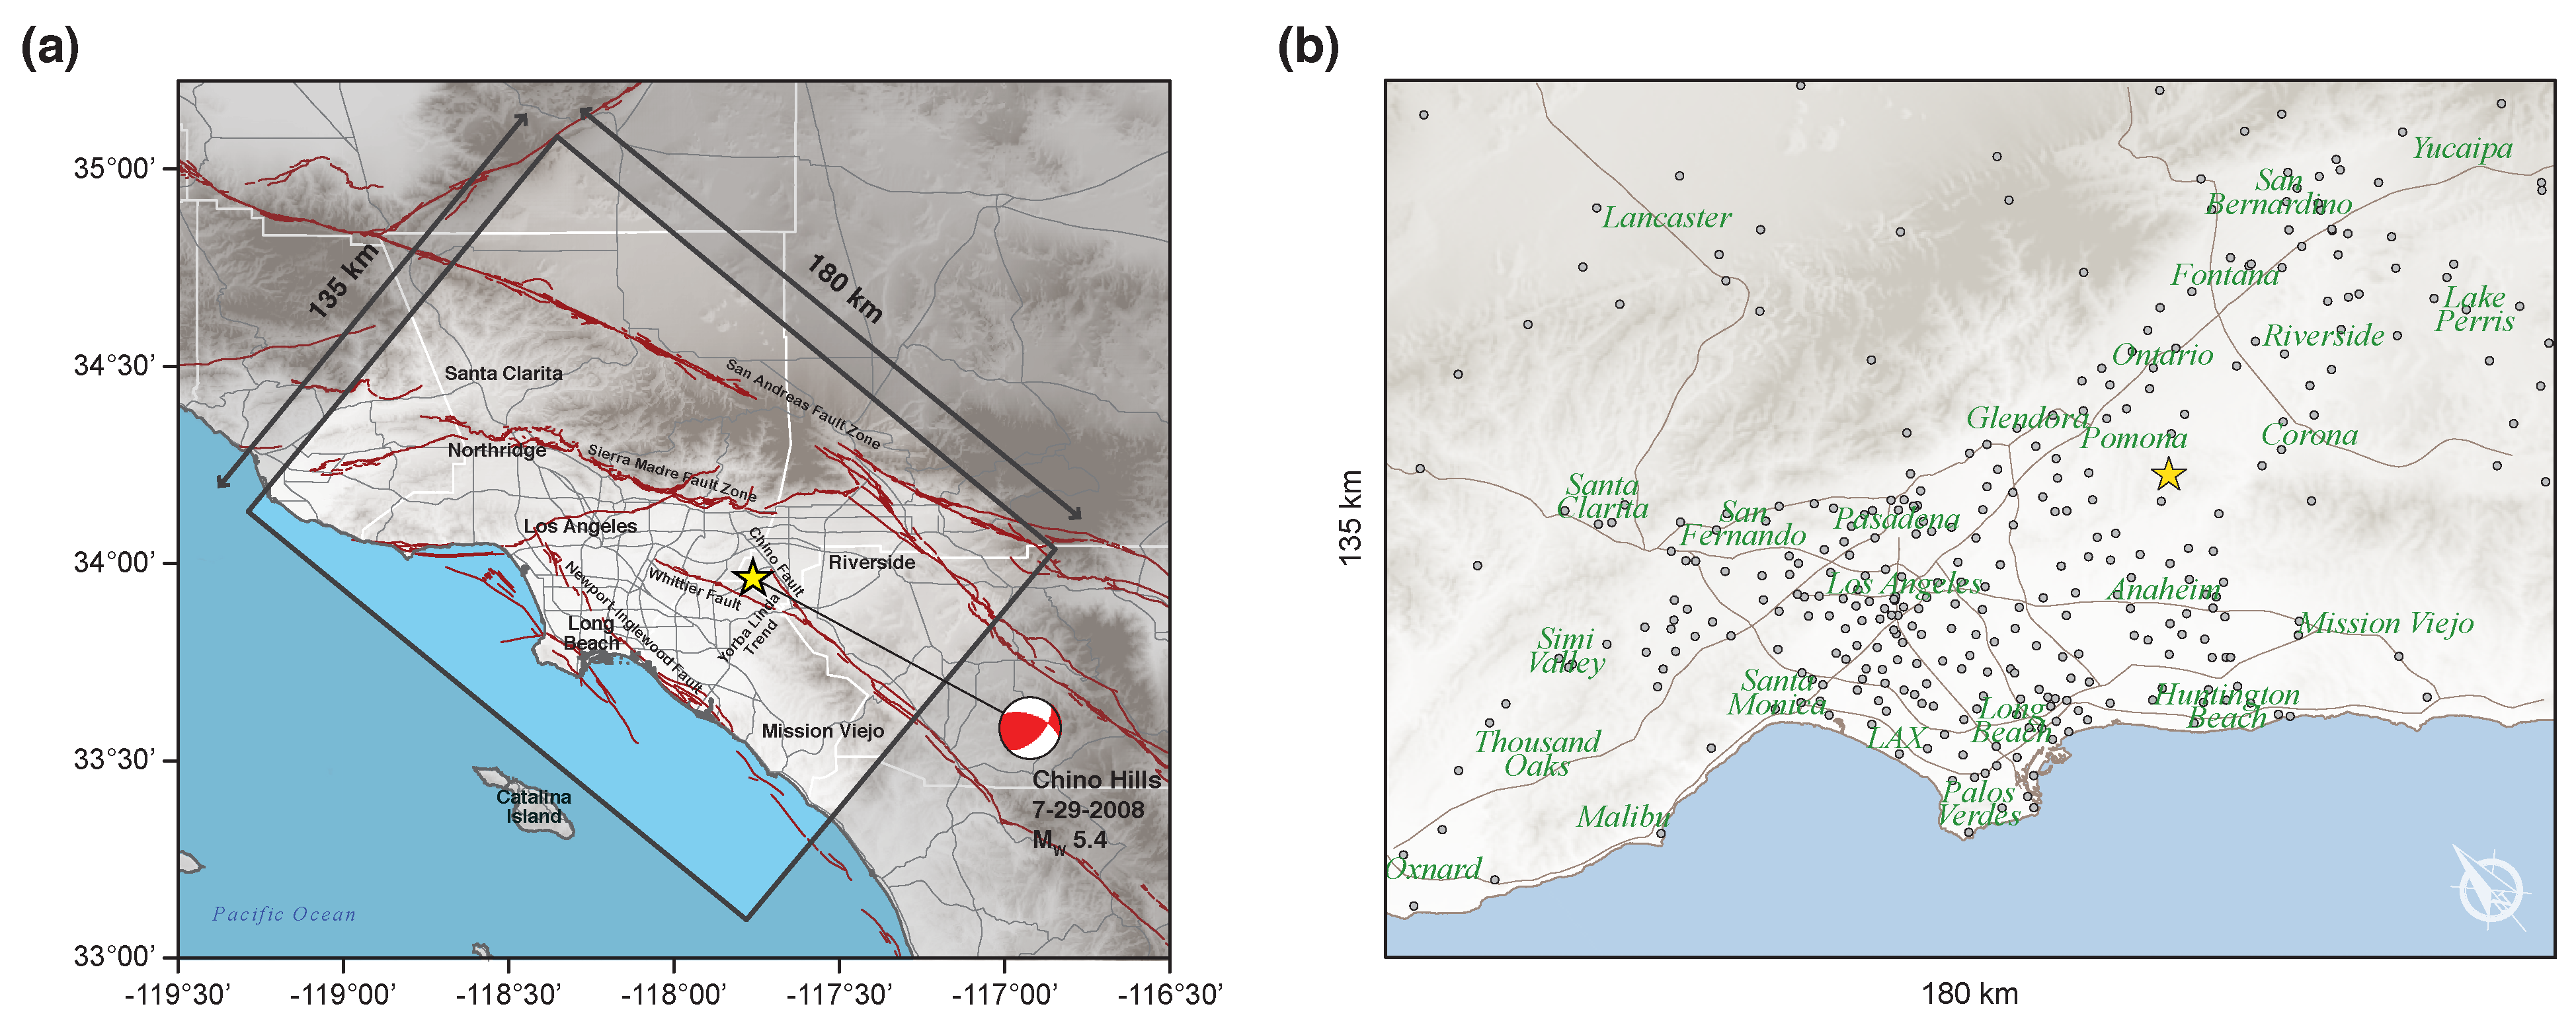
\includegraphics[width=\textwidth]{figures/pdf/figure-01}
    \caption{\textbf{(a)} Region of interest used by \citet{Taborda_2014_BSSA} for the simulations of the 2008 $M_W ~ 5.4$ Chino Hills earthquake, including the epicenter, focal mechanism, and major quaternary faults. In the background, the main roads and topography are shown for visual reference. \textbf{(b)} Distribution of the 336 stations (gray dots) used by \citet{Taborda_2014_BSSA} for the validation analysis of their simulations within the modeling domain shown in part (a). Roads, city names, and the hillshade topography are also shown here in the background for reference. The color version of this figure is available only in the electronic edition.}
    \label{fig:chino-hills}
\end{figure*}

\citet{Anderson_2004_Proc} calibrated the results of GOF scores comparing horizontal components of recorded seismograms and other simulations using the first ten metrics (C1 through C10) in Table \ref{tab:metrics}. He concluded that for a typical distribution of the scores, the GOF could be categorized into four groups: poor (for scores from 0 to 4), fair (4 to 6), good (6 to 8), and excellent (for scores from 8 to 10). While this categorization was arguably subjective, over the years it has become common practice and has been adopted or matched by alternative validation methods \citep[e.g.,][]{Kristekova_2009_GJI, Olsen_2010_SRL}, making the method itself a reference baseline for various validation studies \citep[e.g.,][]{Chaljub_2010_BSSA, Bielak_2010_GJI, Guidotti_2011_SRL, Maufroy_2015_BSSA}.

Here, we focus our analysis on the eleven metrics included in Table \ref{tab:metrics}, and investigate the relationships that exist between them in order to prioritize a reduced number of metrics that can help predict the outcome category one would use to label the results of a given simulation.

% ===========================================================================================
%
% OLD NAEEM VERSION
% 
% Following the guidelines suggested by \citet{Anderson_2004_Proc}, \citet{Taborda_2014_BSSA} applied the scoring procedure to each pair of data and synthetic using compatible broadband sets, and series of bandpass filtered versions of the signals or sub-bands, SB1, SB2, SB3, SB4, and SB5. The signals bandpass filtered between 0.1 and 4 Hz for BB, and between 0.1 Hz and 0.25 Hz, and 0.25 and 0.5 Hz, and 0.5 and 1 Hz, and 1 and 2 Hz, and 2 and 4 Hz for SB1, SB2, SB3, SB4, and SB5, respectively. They also reported a scaled combination score of metrics and bands. However, since the combined scores are linear scaled combinations of metrics and frequency bands, in this specific study, they do not add new information to the data base.  \citet{Khoshnevis_2015_Proc} studied the effect of filtering on GOF score and presented that filtering approach can affect the GOF score and change the final classes. Therefore, in order to avoid extra source of uncertainty in the study, we only consider broadband GOF scores ($0.1-4~Hz$). Analysis of effect of bands in the results could be an appropriate subject for another study. 




% Accuracy of ground motion simulation is evaluated based on a quantitative validation of the simulation ground motions. The validation process consist of comparisons between synthetics and data, at locations where records were available for the simulated events. For validating the simulation of strong motion complex time series, different metrics are defined. These metrics evaluate the similarity of two signals in time or frequency domain. \\

% \citet{Anderson_2004_Proc} proposed 10 individual quality measures to evaluate the credibility of synthetic seismograms.  He proposed to apply the metrics on 10 frequency bands with logarithmic spacing. The logarithmic spacing puts more emphasis on lower frequencies where these frequencies are more amenable to waveform fitting and are particularly important for response of large structures. A comprehensive score (S1) could be achieved by the average of the scores of seismograms filtered in each of the valid frequency bands individually, as well as the broadband seismogram. An alternative score (S2) is obtained by averaging the scores on the ten individual criteria for only the accelerogram filtered to allow all frequencies to pass. \citet{Anderson_2004_Proc} scaled the scores into range of 0 to 10 with 10 giving perfect agreement. He suggested to consider a score below 4 as a poor fit, a score of 4-6 as a fair fit, a score of 6 to 8 as a good fit, and a score over 8 is an excellent fit. However, some of these metrics like integral measures are potentially very easy to fit and some of them like cross correlation is by far the most difficult of all parameters to achieve high score. Therefore, for a pair of synthetic and data some of metrics could belong to good and some of them could belong to fair fit classes.\\

% In other study, \citet{Kristekova_2006_BSSA} developed quantitative misfit criteria for comparison of seismograms. The misfit criteria are defined based on the time-frequency (TF) representation of the seismograms obtained at the continues wavelet transform. Based on local TF envelop and phase differences, they defined envelop and phase misfit dependent on both time and frequency. With projection of TF misfit onto frequency or time domain, they computed frequency- or time-dependent misfits, respectively. The method proposed  by \citet{Kristekova_2006_BSSA} needs to consider one of signals as a reference signal. Therefore, \citet{Kristekova_2009_GJI} presented an extension of the theory of the TF misfit criteria. They defined locally and globally normalized TF criteria where locally normalized misfits can be used if it is important to investigate relatively small part of the signal. The globally normalized misfits can be used for quantifying an overall level of disagreement. In the extended version of the metrics, they defined a misfit criteria for 3 components of a signal and also they developed TF GOF criteria for more realistic scenario where there is a high level of disagreement and it is not possible to consider one of signals as a reference signal. They classified the GOF scores as poor, fair, good, and excellent based on GOF numerical values.\\

% \citet{Olsen_2010_SRL} argued that the \citet{Kristekova_2006_BSSA,Kristekova_2009_GJI}  metrics are suitable for low frequency signals. Therefor, they proposed a new GOF method for validation of Broadband synthetics. They used some of metrics that are used by \citet{Anderson_2004_Proc}, however, they used different scoring approach which generates a relatively high-resolution representation of small misfits. They also used inelastic and elastic response spectra ration (IE ratio) as a structural engineering specific metric. They proposed to combine the metrics for final decisions based on user defined application-based weights.\\

% Recently, \citet{Taborda_2013_BSSA} conducted a simulation for 2008 Chino Hills earthquake and proposed a minor modification in the \citet{Anderson_2004_Proc} metrics. They added an eleventh parameter to the Anderson's scores as strong motion duration.\\

% A comprehensive validation approach should include metrics in both time and frequency domain. All mentioned metrics \citep[i.e.,][]{Anderson_2004_Proc,Kristekova_2006_BSSA,Kristekova_2009_GJI,Olsen_2010_SRL} have this characteristic. However, in this study we are mostly dependent on available data based on \citet{Taborda_2014_BSSA} where they used the GOF method proposed by \citet{Anderson_2004_Proc}, with minor modification introduced by \citet{Taborda_2013_BSSA}. The method compares synthetics against data using 11 individual parameters, namely: Arias Intensity Integral (C1), Energy Integral (C2), Arias Intensity Value (C3), Total Energy (C4), Peak Acceleration (C5), Peak Velocity (C6), Peak Displacement (C7), Response Spectra (C8), Fourier Amplitude Spectrum (C9), Cross Correlation (C10), and Strong Phase Duration (C11). Each parameter is mapped on to a numerical scale ranging from 0 to 10, where a score of 10 corresponds to a perfect  match between two signals.\\
% Following the guidelines suggested by \citet{Anderson_2004_Proc}, \citet{Taborda_2014_BSSA} applied the scoring procedure to each pair of data and synthetic using compatible broadband sets, and series of bandpass filtered versions of the signals or sub-bands, SB1, SB2, SB3, SB4, and SB5. The signals bandpass filtered between 0.1 and 4 Hz for BB, and between 0.1 Hz and 0.25 Hz, and 0.25 and 0.5 Hz, and 0.5 and 1 Hz, and 1 and 2 Hz, and 2 and 4 Hz for SB1, SB2, SB3, SB4, and SB5, respectively. They also reported a scaled combination score of metrics and bands. However, since the combined scores are linear scaled combinations of metrics and frequency bands, in this specific study, they do not add new information to the data base.  \citet{Khoshnevis_2015_Proc} studied the effect of filtering on GOF score and presented that filtering approach can affect the GOF score and change the final classes. Therefore, in order to avoid extra source of uncertainty in the study, we only consider broadband GOF scores ($0.1-4~Hz$). Analysis of effect of bands in the results could be an appropriate subject for another study. 










